%%%%%%%%%%%%%%%%%%%%%%%%%%%%%%%%%%%%%%%%%%%%%%%%%%%%%%%%%%%%%%%%%%%%%%%%%%%%%%%
% Author:  Pablo Alvarado
%
% Escuela de Ingeniería Electrónica
% Instituto Tecnológico de Costa Rica
%
% Tesis de Licenciatura
% 
% Phone:   +506 550 2106
% Fax:     +506 591 6629
% email:   palvarado@ietec.org
%
% $Id: main.tex 1513 2010-08-15 01:25:24Z palvarado $
%
%%%%%%%%%%%%%%%%%%%%%%%%%%%%%%%%%%%%%%%%%%%%%%%%%%%%%%%%%%%%%%%%%%%%%%%%%%%%%%%

% \documentclass is book
\documentclass[12pt,twoside,letterpaper,usenames,dvipsnames]{book}
\usepackage[utf8]{inputenc}
\usepackage{ifthen}                     % provide if-then-else operators
\usepackage{tikz}
\usetikzlibrary{shapes.geometric, arrows}
\usepackage{pgfplots}
\usetikzlibrary{plotmarks}
\usepackage{algpseudocode}
\usepackage{pdfpages}

\tikzstyle{startstop} = [rectangle, rounded corners, minimum width=3cm, minimum height=1cm,text centered, draw=black]
\tikzstyle{io} = [trapezium, trapezium left angle=70, trapezium right angle=110, minimum width=3cm, minimum height=1cm, text centered, draw=black]
\tikzstyle{process} = [rectangle, minimum width=3cm, minimum height=1cm, text centered, text width=3cm, draw=black]
\tikzstyle{decision} = [diamond, minimum width=3cm, minimum height=1cm, text centered, draw=black]
\tikzstyle{arrow} = [thick,->,>=stealth]

% --------------------------------------------------------------------------
% Global variables required in document formatting
% --------------------------------------------------------------------------
%
% BOOK MODE
%
\newboolean{bookmode}                  % boolean used to control book format
% Ensure that only one of the next two lines is active:
\setboolean{bookmode}{true}           % turn book mode on
%\setboolean{bookmode}{false}           % turn book mode off

%
% DRAFT MODE
%
\newboolean{draftmode}                  % boolean used to control draft-mode
% Ensure that only one of the next two lines is active:
\setboolean{draftmode}{false}            % turn draft mode on
%\setboolean{draftmode}{false}           % turn draft mode off
% --------------------------------------------------------------------------
%
% GENERAL AUTHOR, TITLE AND KEYWORDS
%
% Nombre del Estudiante
\newcommand{\scriptAuthor}{Manuel Zumbado Corrales}

% Título de la tesis
\newcommand{\scriptTitle}{Implementaci\'on paralela de optimizaciones computacionales del filtro DNLM para la plataforma Xeon Phi} 

% Keywords
\newcommand{\scriptKeywords}{Non Local Means, Procesamiento de im\'agenes, Paralelizaci\'on, Costo Computacional, Optimizaci\'on, Xeon Phi Knights Landing}

% Descripción de la editorial
\newcommand{\boxeditorial}{%
}

% Para el PDF (cambiar si se desea otras cosas a lo indicado arriba
\newcommand{\pdfAuthor}{\scriptAuthor}
\newcommand{\pdfTitle}{\scriptTitle} 
\newcommand{\pdfKeywords}{\scriptKeywords}

% --------------------------------------------------------------------------

% include all packages and define all required general macros
\input{macros}

% allow equations to be splitted (breaked) into several pages
\allowdisplaybreaks[3]

% --------------------------------------------------------------------------
\begin{document}
  % where to look for graphics
  \graphicspath{{./}{./fig/}}

  \pagenumbering{alph}
  % fix some terms not activated due to the bug of hyperref with spanish.
  \renewcommand{\tablename}{Tabla}
  \renewcommand{\listtablename}{\'Indice de tablas}
  \renewcommand{\examplesolution}{Solución}
  \pagestyle{empty}

  % select one of the following titlepages
  \include{titlepage_licce_es}  % Titlepage in Spanish
  %\include{titlepage_licel_es} % Titlepage in Spanish
  %\include{titlepage_licce_en} % Titlepage in English (only if thesis is in En)
  %\include{titlepage_msc_es}   % Titlepage in Spanish
  %\include{titlepage_msc_en}   % Titlepage in English (only if thesis is in En)

  \include{disclaimer}
  %% ESTE ARCHIVO DEBE ELIMINARSE DE LA VERSIÓN FINAL

\thispagestyle{empty}

%%
%% Indique los nombres de los lectores y asesor
\newcommand{\lectorI}{Dra.\, María del Pilar Pérez Fernández}
\newcommand{\lectorII}{Dr.\,Juan Pérez Hernández}
\newcommand{\director}{Dr.\,Pablo Alvarado Moya}
%% Revise además que 


\begin{center}
  \begin{tabular}{c}
    Instituto Tecnológico de Costa Rica \\
    Escuela de Ingeniería Electrónica \\
    Tesis de Maestría \\
    Tribunal Evaluador
  \end{tabular}
\end{center}

\vfill

Tesis de maestría defendida ante el presente Tribunal Evaluador como
requisito para optar por el grado académico de maestría, del Instituto
Tecnológico de Costa Rica.

\vfill

\vspace*{20mm}
\begin{center}
 Miembros del Tribunal
\end{center}
\vspace*{8mm}

\vfill

\begin{center}
  \begin{tabular}{ccc}
    \rule{70mm}{0.5pt} & \rule{15mm}{0pt} & \rule{70mm}{0.5pt} \\
    \lectorI && \lectorII \\
    Profesora Lectora && Profesor Lector
  \end{tabular}
  
  \vspace{10mm}

  \begin{tabular}{c}
    \rule{6cm}{0.5pt} \\
    \director \\
    Profesor Asesor
  \end{tabular}
\end{center}

\vfill


Los miembros de este Tribunal dan fe de que la presente tesis de maestría 
ha sido aprobada y cumple con las normas establecidas por la Escuela de
Ingeniería Electrónica.

\vfill

\begin{center}
  Cartago, 29 de noviembre de 2011\par
\end{center}

\cleardoublepage

%%% Local Variables: 
%%% mode: latex
%%% TeX-master: "main"
%%% End: 
  % Remover en versión final
  \include{acta}      % Remover en versión final
  \chapter*{Resumen}
\thispagestyle{empty}

En este trabajo se presenta una optimizaci\'on computacional novedosa del filtro deceived non local means usando media m\'ovil y simetr\'ia en el pesado. Se realiza la evaluaci\'on de la optimizaci\'on propuesta con distintos enfoques para disminuir el costo computacional del filtro deceived non local means. Adem\'as, tambi\'en se comprueba el impacto de paralelizar los enfoques de optimizaci\'on, evaluando el tiempo de ejecuci\'on y la escalabilidad en una arquitectura many-core. El enfoque propuesto para la implementaci\'on secuencial alcanza una aceleraci\'on de $90$, mientras que su contraparte paralela alcanza un speedup de $665$ en una imagen de entrada de $1024\times1024$.

\bigskip

\textbf{Palabras clave:} \scriptKeywords

\clearpage
\chapter*{Abstract}
\thispagestyle{empty}

This work presents a novel computational optimization of the deceived non local means filter using moving average and symmetric weighting. Comprise an evaluation of the proposed optimization with different approaches to lower the computational cost of the deceived non local means filter. Furthermore, also assess the impact of parallelizing the different optimization approaches, evaluating the execution time and scalability in a many-core architecture. The proposed approach for the non-parallel implementation achieved a $90$ speedup, while its parallelized counterpart yielded a $665$ speedup with a $1024\times1024$ input image. 

\bigskip

\textbf{Keywords:} Non Local Means filter, Image Processing, Parallelization, Computational Cost, Optimization, Xeon Phi Knights Landing.

\cleardoublepage

%%% Local Variables: 
%%% mode: latex
%%% TeX-master: "main"
%%% End: 

  \vspace*{0.4\textheight}
{\hfill{\Large{\emph{a mis queridos padres, a Diana, Luciano, Abril y al pueblo de Costa Rica por hacer esto posible}}}}

  \chapter*{Agradecimientos}
\thispagestyle{empty}

EN CONSTRUCCION

\vspace*{1cm}

\scriptAuthor

Cartago, \today

\cleardoublepage

%%% Local Variables: 
%%% mode: latex
%%% TeX-master: "paMain"
%%% End: 


  %----------------------------------------------------------------------------
  \frontmatter
  %----------------------------------------------------------------------------
  \pagestyle{fancy}
  \pagenumbering{roman}

  \pdfbookmark[1]{Indice General}{Indice General}

  \parskip0ex                           % space between paragraphs

  \tableofcontents                                      % Table of contents
  \listoffigures                                        % List of figures
  \listoftables                                         % List of tables

\ifdraft{%
  % todo's                                              % TODOs
  \listoftodo
}{%
}

  \include{notation}                                    % Notation
  %% ---------------------------------------------------------------------------
%% paNotation.tex
%%
%% Notation
%%
%% $Id: paNotation.tex,v 1.15 2004/03/30 05:55:59 alvarado Exp $
%% ---------------------------------------------------------------------------

\cleardoublepage
\renewcommand{\nomname}{Lista de símbolos y abreviaciones}
\markboth{\nomname}{\nomname}
\renewcommand{\nompreamble}{\addcontentsline{toc}{chapter}{\nomname}%
\setlength{\nomitemsep}{-\parsep}
\setlength{\itemsep}{10ex}
}

%%
% Símbolos en la notación general
% (es posible poner la declaración en el texto
%%



%%
% Algunas abreviaciones
%%

\syma{FFT}{Transformada R\'apida de Fourier}
\syma{DNLM-MOAS}{Filtro Deceived Non Local Means con Media Movil y Simetr\'ia} 
\syma{DNLM-IIFFT}{Filtro Deceived Non Local Means con Im\'agenes Integrales y FFT} 
\syma{CPU}{Unidad Central de Procesamiento} 
\syma{VPU}{Unidad de Procesamiento Vectorial} 
\syma{USM}{Filtro \engl{Unsharp Mask}} 
\syma{MCDRAM}{Memoria de Alto Ancho de Banda}

\printnomenclature[20mm]

%%% Local Variables:
%%% mode: latex
%%% TeX-master: "paMain"
%%% End:
                                    % Abbreviation

  \parskip1.3ex                           % space between paragraphs

  %----------------------------------------------------------------------------
  \mainmatter
  %----------------------------------------------------------------------------
  % where to look for graphics
  \graphicspath{{./}{./fig/}}
  %\pagenumbering{arab}

  % Main files
  %% ---------------------------------------------------------------------------
%% intro.tex
%%
%% Introduction
%%
%% $Id: intro.tex 1477 2010-07-28 21:34:43Z palvarado $
%% ---------------------------------------------------------------------------

\chapter{Introducción}
\label{chp:intro}

%En la \nt{introducción} deben quedar completamente claros los siguientes
%aspectos, cuyo significado depende del tipo concreto de tesis:
%
%\begin{compactitem}
%\item Contexto
%\item Problema
%\item Esbozo de solución
%\item Objetivos y estructura
%\end{compactitem}
%
%El contexto corresponde al entorno donde se desarrolla el proyecto de
%tesis, que puede ser el área general de aplicación, un dominio de
%problemas, etc. El problema concreto se sintetiza usualmente en una
%frase o pregunta. Esta pregunta debería ser una consecuencia a la que
%se llega después de realizar el desarrollo del contexto. Del
%planteamiento del problema se deriva cuál es el objetivo del trabajo
%en particular, que a su vez debe conducir al lector de forma natural
%al esbozo de la solución del problema a tratar en la
%tesis. Generalmente para aclarar la solución se hace uso de un
%diagrama de bloques o diagrama de flujo general, es decir, desde un
%nivel de abstracción alto, donde no sea necesario entrar en detalles
%técnicos. Usualmente este diagrama y su breve explicación dictan cuál
%debe ser la estructura del resto del tesis, que es mencionada siempre
%al final de la introducción.
%
%Una buena introducción debe lograr que el lector tenga interés de leer el resto
%del tesis.
%
%Es recomendable dividir la tesis en secciones, nombradas cada una de acuerdo a
%su contenido. \textbf{Jamás} utilice los nombres de la guía como
%``\emph{Problema existente e importancia de su solución}'', sino algo como ``La
%deforestación en Costa Rica'' o lo que se adecúe a su problema en particular.
%
%Recuerde que en español solo la primera letra del título va en mayúscula
%(exceptuando nombres propios, por supuesto).

El mejoramiento de las im\'agenes es un proceso en el que por medio de diferentes t\'ecnicas se obtiene un realce de las caracter\'isticas o informaci\'on relevante y la atenuaci\'on de informaci\'on poco importante o no deseada. Esto permite mejorar la efectividad de m\'etodos de segmentaci\'on, rastreo de objetos, clasificaci\'on y otras t\'ecnicas de reconocimiento de patrones y el aprendizaje autom\'atico. 


Los filtros espaciales son ampliamente utilizados para la reducci\'on de los diferentes tipos de ruido encontrados en las im\'agenes. Muchas veces se emplean en combinación con t\'ecnicas como la ecualizaci\'on de histogramas, que permite obtener una mejora en el contraste; o Unsharp Masking (USM) para resaltar los bordes.

Uno de los filtros con mejor resultado en la reducción de ruido es el Non-Local Means (NLM) propuesto en \textcite{1467423}, ya que se basa en la similitud entre los vecindarios de los pixeles contenidos en una ventana de búsqueda deslizante para el ponderamiento del peso asignado a cada pixel. Este enfoque ha demostrado muy buenos resultados con una menor p\'erdida de detalles (como por ejemplo los bordes) en comparaci\'on con otros filtros como el de mediana y el bilateral \cite{calderon2016first}. Es importante resaltar que este algoritmo es altamente paralelizable, debido a que no existe dependencia en el c\'alculo de los pixeles que componen la imagen. 

Existen mejoras desarrolladas a partir del algoritmo NLM, un enfoque novedoso es el propuesto en \textcite{7160148} llamado Deceived Non-Local Means (DNLM). Presenta una combinaci\'on del m\'etodo Unsharp Masking (USM) con el filtro NLM por medio del desacoplamiento de la imagen utilizada en el pesado y la imagen usada en el filtrado. Esto permite reducir los artefactos no deseados en las im\'agenes (efecto de anillo) generados por el enfoque convencional, es decir, al aplicar primero el m\'etodo USM y posteriormente el filtro NLM.  

Uno de los principales inconvenientes del filtro NLM es su complejidad computacional: En el peor de los casos, para una imagen de entrada de $N$ pixeles utilizando un tamaño de ventana deslizante de $A\times B = N$ y un tamaño de vecindario de $A\times B = N$, la complejidad computacional es de $\mathcal{O}(N^{3})$. 

Lo anterior provoca que el tiempo de procesamiento del filtro NLM sea una limitante importante a considerar, en especial si se planea utilizar para una tarea en tiempo real o en el preprocesado de grandes vol\'umenes de im\'agenes (en el caso de sets de datos para aprendizaje autom\'atico). 

Una forma de reducir la complejidad computacional del filtro es mediante el uso de optimizaciones o aproximaciones del algoritmo. Este proyecto pretende continuar el trabajo realizado previamente, que consisti\'o en el desarrollo de una propuesta de optimizaci\'on para el filtro DNLM por medio del uso de Im\'agenes Integrales y la Transformada R\'apida de Fourier (DNLM-IIFFT). Esta optimizaci\'on permite reducir la complejidad del algoritmo a  $\mathcal{O}(N^{2}\log(N))$. Los resultados experimentales arrojan una aceleraci\'on de hasta 10 veces en el procesamiento de una imagen de 720p. Si bien estos resultados presentan una aceleraci\'on importante, se deben explorar t\'ecnicas de paralelizaci\'on que permitan reducir a\'un m\'as el tiempo de ejecuci\'on del algoritmo. 

\begin{figure}[htb]
  \centering
  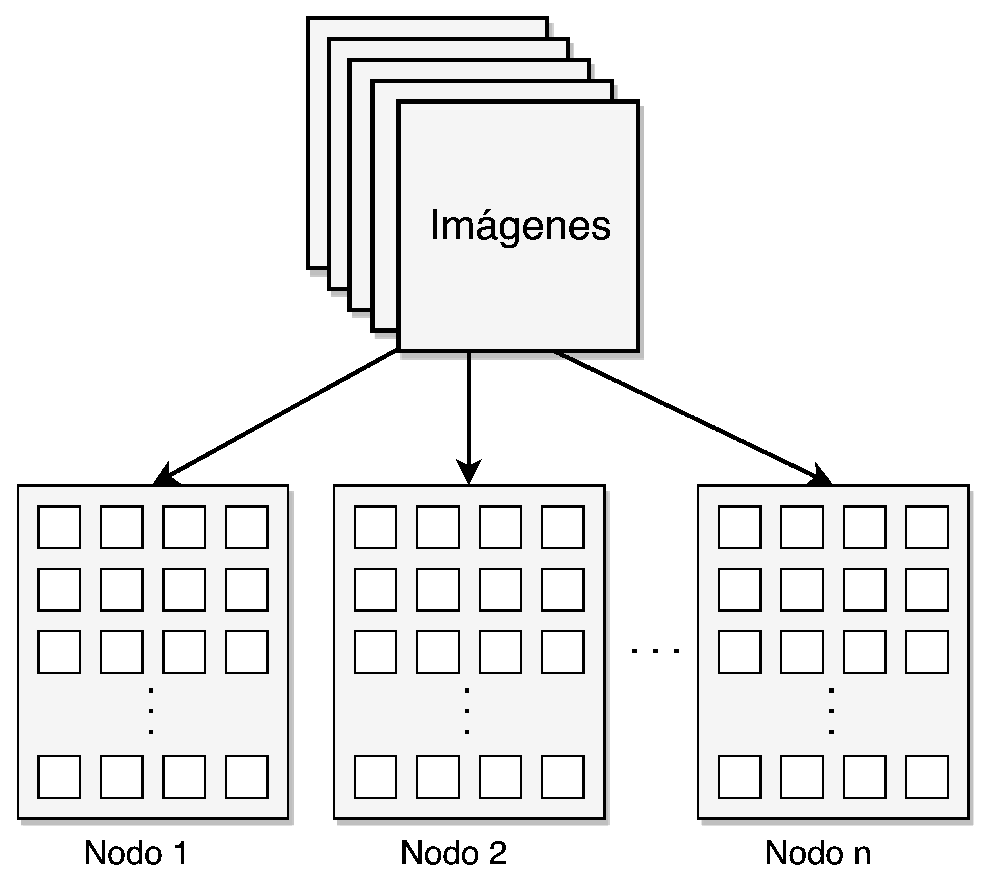
\includegraphics[width=0.9\textwidth]{blockD}
  \caption{Diagrama de bloques de la soluci\'on}
  \label{fig:ltxfig}
\end{figure}

*COMENTAR Y HACER REFERENCIA SOBRE FIGURA*

\section{Objetivos y estructura del documento}

\index{objetivos}

Este trabajo tiene como objetivo la paralelizaci\'on del filtro DNLM-IIFFT optimizado para la arquitectura Xeon Phi Knights Landing, que permita el procesamiento eficiente de grandes vol\'umenes de im\'agenes.
En este trabajo se realiza una implementaci\'on paralela del filtro DNLM-IFFT (modificaci\'on del filtro NLM) en sistemas multi-nodo optimizados para la arquitectura Intel Knights Landing, con la finalidad de realizar procesamiento concurrente y de alto rendimiento de grandes conjuntos de im\'agenes. 



%Esta plantilla LaTeX tiene como objetivo simplificar la construcción del
%documento de tesis, presentando ejemplo de figuras y tablas, así como otorgar
%una plataforma de compilación en GNU/Linux que simplifique la administración de
%todo el documento.
%
%La última sección de la introducción usualmente sí tiene un título estandar que
%es ``Objetivos y estructura del documento'', donde se presentan \emph{en prosa}
%los objetivos general y específicos que ha tenido el proyecto de tesis,
%así como la estructura de la tesis (por ejemplo, ``en el siguiente capítulo se
%esbozan los fundamentos teóricos necesarios para explicar en el
%capítulo~\ref{ch:solucion} la propuesta realizada$\ldots$''

%%% Local Variables: 
%%% mode: latex
%%% TeX-master: "main"
%%% End: 

  \chapter{Marco teórico}
\label{ch:marco}


En este capítulo se detalla el contenido teórico necesario para el desarrollo de este trabajo. La propuesta consiste en la optimización y paralelización del filtro \engl{Deceived Non-Local Means} (DNLM). Este filtro es una modificación del filtro \engl{Non-Local Means} (NLM) que adiciona la mejora de bordes y contraste, conservando la preservación de bordes y la robustez ante el ruido proporcionada por el filtro NLM \cite{calderon2015dewaff}. 
Las optimizaciones computacionales del filtro NLM se pueden agrupar en dos enfoques: Optimizaciones exactas y aproximaciones del algoritmo. Existen propuestas de optimización del rendimiento del filtro NLM en términos del ruido eliminado, sin embargo se emplean técnicas de clústering, diccionarios y otros métodos probabilísticos para preclasificar parches similares en la imagen, a\~nadiendo complejidad computacional al procesamiento \cite{pardoNLM:2018,Chan2013,Tasdizen2009,Chatterjee2008,JI20091238,Karam2018}. 
La propuesta de paralelización incluye la evaluación de dos optimizaciones computacionales exactas del filtro NLM adaptadas al filtro DNLM: DNLM-IIFFT y DNLM-MA.



\section{Eliminación de ruido}

\subsection{Ruido Blanco Aditivo de distribución Gaussiana}
\label{ch:marco_agwn}

El ruido presente en im\'agenes se debe a fenómenos naturales en el proceso de captura, transmisión y almacenamiento de las im\'agenes. 	Una forma de modelar este ruido es mediante el ruido blanco aditivo de distribución gaussiana. Este ruido es llamado gaussiano porque se modela a través de una distribución de probabilidad gaussiana. Se dice que es blanco debido a que su espectro de intensidad es plano. Se le llama aditivo porque la distorción causada por el ruido se modela a través de la suma del ruido a los pixeles de la imagen. El modelo de ruido gaussiano  est\'a dado por:

\begin{equation}
\label{eq:modelruido}
U = X + V \enspace ,
\end{equation}

 donde $U$ es la imagen con ruido gaussiano, $X$ corresponde a la imagen sin ruido y $V$ corresponde a una variable alatoria que sigue una función de densidad de probabilidad gaussiana dada por: 
 
\begin{equation}
\label{eq:probfuncgauus}
p(v(x)) = \frac{1}{{\sigma \sqrt {2\pi } }}e^{{{ - \left( {v(x) - \mu } \right)^2 } \mathord{\left/ {\vphantom {{ - \left( {x - \mu } \right)^2 } {2\sigma ^2 }}} \right. \kern-\nulldelimiterspace} {2\sigma ^2 }}} \enspace ,
\end{equation}

siendo $\sigma$ la desviación est\'andar  y $\mu$ el valor medio de la distribución de probabilidad, que para efectos del ruido gaussiano se asume $\mu = 0$.


\section{Filtro Non-Local Means}
\label{ch:marco_nlm}

El filtro NLM forma parte de los filtros espaciales de promedio ponderado que pueden definirse de manera general como:

\begin{equation}
\label{eq:weighted}
Y(U,p)=\left(\sum_{m\in \Omega}\psi\left(U, p, m\right)\right)^{-1} \\ \left(\sum_{m\in \Omega}\psi\left(U, p, m\right)U(m)\right) \enspace ,
\end{equation}

donde $p$ es el pixel que se pretende filtrar, $m$ corresponde a un pixel contenido en la ventana deslizante $\Omega$, $\psi$ es una función de pesado del filtro y $U$ la imagen de entrada \cite{calderon2015dewaff}.

La función de pesado del filtro NLM se define como:

\begin{equation}
\label{eq:nlmfunc}
\psi_{\textrm{NLM}}\left(U,p,m\right) = \exp\left(-\frac{\left\Vert \vec{\boldsymbol{\eta}}\left(m\right)-\vec{\boldsymbol{\eta}}\left(p\right)\right\Vert^2 }{h}\right) \enspace ,
\end{equation}

donde $h$ es el par\'ametro que controla el grado de suavizado del filtro con $h = \alpha\sigma^{2}$; y $\vec{\boldsymbol{\eta}}\left(q\right)$ el vector que contiene los pixeles de un vecindario de tama\~no $W$ al rededor de $q$, con $q \in \{p,m\}$.

Este filtro introduce el concepto de similitud entre vencindarios de pixeles y no entre sus intensidades, como en otros filtros. La función de pesado definida en (\ref{eq:nlmfunc}) hace uso de la distancia Euclidiana para determinar la similitud entre los vecindarios de los pixeles $p$ y $m$. 
De esta manera se determina el peso en la contribución para el ponderamiento de los pixeles en una región limitada por una ventana $\Omega$. Este enfoque reduce los cambios bruscos en la intensidad de pixeles aleda\~nos al comparar los vecindarios en un \'area local, a la vez que permite conservar detalles como bordes y patrones en la imagen\cite{calderon2015dewaff}. 


En cuanto a la complejidad computacional, al filtrar una imagen de entrada en escala de grises de $N$ pixeles, con una ventana deslizante de tama\~no $|\Omega| = S$ pixeles y un vecindario de tama\~no $W$ pixeles, la complejidad computacional del filtro DNLM es de $\mathcal{O}(N\cdot~S\cdot~W)$. 



\section{Mejora de bordes y contraste}

\subsection{Unsharp Masking}
\label{ch:marco_usm}

Los métodos de Unsharp Masking se utilizan para el realce de los bordes y la mejora de contraste en las im\'agenes. Se realiza mediante una substracción de la imagen suavizada a la imagen original. Esto origina una imagen $B$ con las frecuencias altas de la imagen, es decir, los bordes y otros cambios de intensidad bruscos en los pixeles típicamente representados como detalles y ruido. 

Adicionalmente, se puede emplear un enfoque inverso que consiste en sumar la imagen $B$ con la información de bordes y detalles en alta frecuencia a la imagen original. La adición se controla en una proporción dada por el coeficiente $\lambda$, con:

\begin{equation}
\label{eq:unsharpmask}
G=U+\lambda~B \enspace .
\end{equation}

Por ejemplo, $B$ corresponde a

\begin{equation}
\label{eq:unsharfilter}
B=l*U \enspace 
\end{equation}

y $l$ puede estar dado por:

\begin{equation} l = \left[
\begin{array}{ccc}
1 & 1 & 1\\
1 & -8 & 1\\
1 & 1 & 1
\end{array}\right]
\end{equation}

para el caso de la aproximación al laplaciano.

La imagen $B$ se obtiene por medio de la convolución entre la imagen original y un kernel de aproximación al laplaciano, laplaciano de gaussiano o de diferencia de gaussianas.


En este trabajo se utiliza un kernel de aproximación al laplaciano por medio del laplaciano de gaussiano \cite{sotak1989laplacian}:

\begin{equation}
\label{eq:log}
\operatorname{LoG}(x,y) = \frac{1}{\pi\sigma^4}\left(\frac{x^2+y^2}{2\sigma^2} - 1\right)e^{-\frac{x^2+y^2}{2\sigma^2}},
\end{equation}

La figura \ref{fig:exampleUSM} muestra el resultado de aproximar al laplaciano de una de imagen de entrada y la salida del método USM con la imagen mejorada en contraste y bordes. 

\begin{figure}[H]
%
\begin{minipage}{0.25\textwidth}
  \centering
  \centerline{\includegraphics[width=\linewidth]{lena}}
%  \vspace{1.5cm}
  \centerline{(a) Imagen de entrada $U$.}\medskip
\end{minipage}
\hfill
\begin{minipage}{0.25\textwidth}
  \centering
  \centerline{\includegraphics[width=\linewidth]{lena_lapl}}
%  \vspace{1.5cm}
  \centerline{(b) Laplaciano de $U$.}
\end{minipage}
\hfill
\begin{minipage}{0.25\textwidth}
  \centering
  \centerline{\includegraphics[width=\linewidth]{lena_sharp}}
%  \vspace{1.5cm}
  \centerline{(c) Imagen de salida $U_{\textrm{USM}}$.}\medskip
\end{minipage}
%
\caption[Ejemplo de mejora en imagen con \engl{Unsharp Mask}]{Salida del filtro USM con $\lambda = 5$ y $\sigma = 0.01$. \label{fig:exampleUSM}}
%
\end{figure}


\section{Filtro Deceived Non-Local Means}
\label{ch:marco_dnlm}


El enfoque del filtro \engl{Deceived Non-Local Means} (DNLM) consiste en la combinación de un método de \engl{Unsharp Masking} (USM) con el filtro NLM, con el propósito de lograr por un lado una mejora en los bordes y en el contraste de la imagen, y por otro lado la eliminación del ruido gausiano  presente en la imagen. La combinación propuesta se basa en el desacople entre la imagen usada en el pesado (imagen original $U$) y la utilizada en el filtrado $U_{\textrm{USM}}$. Esto permite evitar el efecto anillo presente en las im\'agenes filtradas con el USM \cite{calderon2015dewaff}.

La función del filtro DNLM est\'a dada por:

\begin{equation}
\label{eq:dnlm}
Y(U,p)=\left(\sum_{m\in \Omega}\psi_{NLM}\left(U, p, m\right)\right)^{-1} \\ \left(\sum_{m\in \Omega}\psi_{\textrm{NLM}}\left(U, p, m\right)U_{\textrm{USM}}(m)\right) \enspace ,
\end{equation}

donde $U$ es la imagen de entrada, $p$ es el pixel que se pretende filtrar, $m$ corresponde a un pixel contenido en la ventana deslizante $\Omega$, $\psi_{\textrm{NLM}}$ es una función de pesado del filtro NLM y $U_{\textrm{USM}}$ la imagen producto de la mejora con el método USM \cite{calderon2015dewaff}. El desacople mostrado en (\ref{eq:dnlm}) se da al realizar el c\'alculo de los pesos con la imagen de entrada $U$ y el filtrado con la imagen $U_{\textrm{USM}}$.

La figura \ref{fig:exampleDNLM} muestra el aumento en contraste de la imagen y el mayor detalle en bordes resultado del procesamiento con el filtro DNLM.

\begin{figure}[H]
\centering
\begin{minipage}[b]{0.3\textwidth}
  \centering
  \centerline{\includegraphics[width=\linewidth]{512x512}}
%  \vspace{1.5cm}
  \centerline{(a) Ejemplo de imagen de actividad celular.}\medskip
\end{minipage}
\hfill
\begin{minipage}[b]{0.3\textwidth}
  \centering
  \centerline{\includegraphics[width=\linewidth]{512x512_DeNLM}}
%  \vspace{1.5cm}
  \centerline{(b) Imagen fitrada.}
\end{minipage}
\vfill
\begin{minipage}[b]{0.3\textwidth}
  \centering
  \centerline{\includegraphics[width=\linewidth]{11043}}
%  \vspace{1.5cm}
  \centerline{(c) Imagen de rayos-x.}\medskip
\end{minipage}
\hfill
\begin{minipage}[b]{0.3\textwidth}
  \centering
  \centerline{\includegraphics[width=\linewidth]{11043_DeNLM}}
%  \vspace{1.5cm}
  \centerline{(d) Imagen filtrada.}\medskip
\end{minipage}
%
\caption[Ejemplo de im\'agenes filtradas con el filtro DNLM]{Ejemplo de im\'agenes filtradas con el filtro DNLM. \label{fig:exampleDNLM}}

%
\end{figure}



\section{Optimizaciones computacionales}
\label{ch:marco_opt}

\subsection{DNLM-IIFFT}
\label{ch:marco_dnlmifft}

Esta optimización computacional utiliza im\'agenes integrales y la transformada r\'apida de Fourier para disminuir la complejidad computacional del filtro DNLM. 



Al analizar la distancia euclidiana $D$ entre los vecindarios se tiene que:

\begin{equation}
D\left(x,y\right)=\left\Vert \vec{\boldsymbol{\eta}}\left(y\right)-\vec{\boldsymbol{\eta}}\left(x\right)\right\Vert^2 \enspace . 
\end{equation}

La ecuación anterior puede representarse en notacion matricial con la norma de Frobenius $\Vert \cdot \Vert_{F}$ como:


\begin{equation}
D\left(x,y\right)=\Vert \mat{Y} - \mat{X} \Vert_{F}^2 \enspace ,
\label{eq:distMat}
\end{equation}

con \mat{Y} y \mat{X} las matrices de los vecindarios de los pixeles $y$ y $x$. respectivamente.

Si se se define la norma $\Vert \cdot \Vert_{F}^2$ con el producto interno de Frobenius $\langle\,\cdot,\cdot\rangle_{F}$ se tiene que:

\begin{equation}\label{eq:frobProd}
\begin{split}
\Vert \mat{Y} - \mat{X} \Vert_{F}^2 & = \langle\mat{Y} - \mat{X},\mat{Y} - \mat{X}\rangle_{F}  \quad \text{y por sesquilinealidad:}\\ 
& = \langle\mat{Y},\mat{Y}\rangle_{F} + \langle\mat{Y},-\mat{X}\rangle_{F} + \langle-\mat{X},\mat{Y}\rangle_{F} + \langle-\mat{X},-\mat{X}\rangle_{F}\\
& = \Vert \mat{Y} \Vert_{F}^2 -2\langle\mat{Y},\mat{X}\rangle_{F} + \Vert \mat{X} \Vert_{F}^2 \enspace ,
\end{split} 
\end{equation}


tomando en cuenta que $\Vert \cdot \Vert_{F}^2$ es una norma que cumple todos los axiomas correspondientes. 

\begin{table}
\begin{center}
\caption{Ejemplo de imagen de entrada \mat{U}.\label{table:imageExample}}

\renewcommand{\arraystretch}{1.4}
\setlength\tabcolsep{3pt}

{
\begin{tabular}{cc|ccc|c}
 & \multicolumn{1}{c}{\textbf{1}} & \textbf{2} & \textbf{3} & \multicolumn{1}{c}{\textbf{4}} & \textbf{5}\tabularnewline
\textbf{1} & \multicolumn{1}{c}{5} & 12 & 1 & \multicolumn{1}{c}{3} & 2\tabularnewline
\cline{3-5} 
\textbf{2} & 5 & 2 & 3 & 1 & 4\tabularnewline
\textbf{3} & 3 & 1 & \textbf{2} & 3 & 1\tabularnewline
\textbf{4} & 4 & 3 & 2 & 1 & 3\tabularnewline
\cline{3-5} 
\textbf{5} & \multicolumn{1}{c}{1} & 5 & 6 & \multicolumn{1}{c}{5} & 3\tabularnewline
\end{tabular}
}
\par\end{center} 
\end{table}

El siguiente ejemplo ilustra el cálculo de la norma de Frobenius entre los vecindarios de pixeles contenidos en la imagen $\mat{U} \in\mathbb{R}^{5 \times 5}$ definida en la Tabla \ref{table:imageExample}. Para efectos de la ilustración, se toman los vecindarios $\mat{P}_{\left(3,3\right)},\mat{P}_{\left(2,2\right)} \in\mathbb{R}^{3\times3}$ de la imagen de ejemplo \mat{U}  y se realiza  el cálculo de la norma de Frobenius tal que:


\begin{equation}
\label{eq:resultado1}
\begin{split}
\left\Vert \mat{P}_{\left(3,3\right)}-\mat{P}_{\left(2,2\right)}\right\Vert_{F} ^{2} & =\left\Vert \left[\begin{array}{ccc}
2 & 3 & 1\\
1 & 2 & 3\\
3 & 2 & 1
\end{array} \right]-\left[\begin{array}{ccc}
5 & 12 & 1\\
5 & 2 & 3\\
3 & 1 & 2
\end{array}\right]\right\Vert_{F}^2 \\
& =\left\Vert\left[\begin{array}{ccc}
-3 & -9 & 0\\
-4 & 0 & 0\\
0 & 1 & -1
\end{array}\right]\right\Vert_{F}^2 \\
& =108 \enspace .
\end{split}
\end{equation}



Al desarrollar (\ref{eq:resultado1}) como se muestra en (\ref{eq:frobProd}), se obtiene que: 
\begin{equation}\label{eq:matFrodProd}
\resizebox{.9 \textwidth}{!} 
{
$\begin{split}
\lVert \mat{P}_{\left(3,3\right)}-\mat{P}_{\left(2,2\right)}\rVert_{F} ^{2} & =\lVert \mat{P}_{\left(3,3\right)}\rVert_{F}^2 -2\langle\mat{P}_{\left(3,3\right)},\mat{P}_{\left(2,2\right)}\rangle_{F} + \lVert \mat{P}_{\left(2,2\right)}\rVert_{F}^2  \\
& = \left\Vert\left[\begin{array}{ccc}
2 & 3 & 1\\
1 & 2 & 3\\
3 & 2 & 1
\end{array}\right]\right\Vert_{F}^2-2\left\langle\left[\begin{array}{ccc}
2 & 3 & 1\\
1 & 2 & 3\\
3 & 2 & 1
\end{array}\right],\left[\begin{array}{ccc}
5 & 12 & 1\\
5 & 2 & 3\\
3 & 1 & 2
\end{array}\right]\right\rangle_{F}
+\left\Vert\left[\begin{array}{ccc}
5 & 12 & 1\\
5 & 2 & 3\\
3 & 1 & 2
\end{array}\right]\right\Vert_{F}^2 \\
& =42+-2\cdot78+222\\
& =42-156+222\\
& =108 \enspace ,
\end{split}$
}
\end{equation}


consistente con los resultados obtenidos en (\ref{eq:resultado1}).




Esta optimización del filtro DNLM se centra en el cálculo de la norma de Frobenius desarrollada en  (\ref{eq:frobProd}) de la siguiente manera:

\begin{itemize}
\item El uso de la imagen integral cuadrática para calcular los términos $\Vert \mat{Y} \Vert_{F}^2 $ y $\Vert \mat{X} \Vert_{F}^2 $.
\item Calcular la convolución para obtener el término $-2\langle\mat{Y},\mat{X}\rangle_{F} $
correspondiente a la correlación del vecindario \mat{Y} con la ventana de búsqueda \mat{\Omega}, para acceder posteriormente al elemento de la matriz resultante en la posici\'on correspondiente.
\end{itemize}

Lo anterior permite disminuir la complejidad computacional del filtro a $\mathcal{O}(S\log(S) \cdot N)$.
 
\subsubsection{Imágenes integrales}


La imagen integral $\mat{I}_{\Sigma}$ de una imagen de entrada \mat{U} presentada en \cite{viola2001robust}, está dada por: 
\begin{equation}
\mat{I}_{\Sigma}\left(x,y\right)=\sum_{i\leq x}\sum_{j\leq y}u_{ij} \enspace ,
\end{equation}
la cual corresponde a la sumatoria de todos los  pixeles ubicados a la izquierda y superiores al pixel $u_{ij}$ de la imagen de entrada \mat{U}.

\begin{table}
\begin{center}
\caption{Ejemplo de imagen de entrada \mat{U^{\odot 2}}.\label{table:imageExample2}}

\renewcommand{\arraystretch}{1.4}
\setlength\tabcolsep{3pt}

{
\begin{tabular}{cc|ccc|c}
 & \multicolumn{1}{c}{\textbf{1}} & \textbf{2} & \textbf{3} & \multicolumn{1}{c}{\textbf{4}} & \textbf{5}\tabularnewline
\textbf{1} & \multicolumn{1}{c}{5} & 12 & 1 & \multicolumn{1}{c}{3} & 2\tabularnewline
\cline{3-5} 
\textbf{2} & 25 & 4 & 9 & 1 & 16\tabularnewline
\textbf{3} & 9 & 1 & \textbf{2} & 9 & 1\tabularnewline
\textbf{4} & 16 & 9 & 4 & 1 & 9\tabularnewline
\cline{3-5} 
\textbf{5} & \multicolumn{1}{c}{1} & 5 & 6 & \multicolumn{1}{c}{5} & 3\tabularnewline
\end{tabular}
}
\par\end{center} 
\end{table}


Continuando con el ejemplo previamente mostrado, la imagen de entrada \mat{U} con sus elementos elevados al cuadrado se define como el producto de Hadamard $\mat{U}^{\odot 2} = \mat{U} \odot \mat{U}$, como se muestra en la tabla \ref{table:imageExample2}. 


\begin{table}
\caption{Imagen integral para $U^{\odot2}$.\label{table:integralcuad}}
\begin{center}
\renewcommand{\arraystretch}{1.4}
\setlength\tabcolsep{3pt}
{
\begin{tabular}{cc|ccc|c}
 & \multicolumn{1}{c}{\textbf{1}} & \textbf{2} & \textbf{3} & \multicolumn{1}{c}{\textbf{4}} & \textbf{5}\tabularnewline
\textbf{1} & \multicolumn{1}{c}{\textbf{25(a)}} & 169 & 170 & \multicolumn{1}{c}{\textbf{179(b)}} & 183\tabularnewline
\cline{3-5} 
\textbf{2} & 50 & 198 & 208 & 218 & 238\tabularnewline
\textbf{3} & 59 & 208 & \textbf{222} & 241 & 262\tabularnewline
\textbf{4} & \textbf{75(c)} & 233 & 251 & \textbf{271(d)} & 301\tabularnewline
\cline{3-5} 
\textbf{5} & \multicolumn{1}{c}{76} & 259 & 313 & \multicolumn{1}{c}{358} & 397\tabularnewline
\end{tabular}
}
\par\end{center}
\end{table}


La imagen integral $\mat{I}_{\Sigma}$ se puede calcular iterativamente para un pixel específico de la imagen de entrada \mat{U} de la siguiente manera: 
\begin{equation}
\mat{I}_{\Sigma}\left(x,y\right)=\mat{U}\left(x,y\right)-\mat{I}_{\Sigma}\left(x-1,y-1\right)+\mat{I}_{\Sigma}\left(x,y-1\right)
+\mat{I}_{\Sigma}\left(x-1,y\right) \enspace ,
\end{equation}

lo cual, para el ejemplo anterior significa que:

\begin{equation}
\mat{I}_{\Sigma}\left(3,3\right)=4-198+208+208=222 \enspace .
\end{equation}

Las imágenes integrales son útiles para calcular la sumatoria sobre una región determinada de la imagen, con una complejidad computacional constante de $\mathcal{O}(1)$. 

Al utilizar la imagen integral $\mat{I}_{\Sigma}$ para calcular la sumatoria de una región de la imagen original \mat{U}, limitada por los pixeles $a=\left(x_{0},y_{0}\right)$,
$b=\left(x_{1},y_{0}\right)$, $c=\left(x_{0},y_{1}\right)$ and $d=\left(x_{1},y_{1}\right)$, ilustrados en la Tabla \ref{table:integralcuad}, se calcula como: 

\begin{equation}
\sum_{i>x_{0}}^{i\leq x_{1}}~\sum_{j>y_{0}}^{j\leq y_{1}}u_{ij}=\mat{I}_{\Sigma}\left(d\right)+\mat{I}_{\Sigma}\left(a\right)-\mat{I}_{\Sigma}\left(b\right)-\mat{I}_{\Sigma}\left(c\right) \enspace ,
\end{equation}

y en el ejemplo presentado para una ventana de $3\times3$ pixeles alrededor del pixel $u_{3,3}^2$ de la imagen $\mat{U}^{\odot2}$ , los pixeles de las esquinas están dados por: $a=\left(1,1\right)$, $b=\left(4,1\right)$,
$c=\left(1,4\right)$ y $d=\left(4,4\right)$, como se muestra en la Tabla \ref{table:imageExample2}. El cálculo de la sumatoria de los pixeles en la región especificada está dada por: 

\begin{equation}
\sum_{i>1}^{i\leq 4}~\sum_{j>1}^{j\leq 4}u_{i,j}^2=271+25-179-75=42 \enspace ,
\end{equation}

lo cual, es consistente con el término $\mat{P}_{\left(3,3\right)}$ en (\ref{eq:matFrodProd}). 



\subsubsection{Convolución y transformada rápida de Fourier}

Como se mostró anteriormente, el término $-2\langle\mat{Y},\mat{X}\rangle_{F}$ producto del desarrollo de la norma de Frobenius en (\ref{eq:matFrodProd}), puede representarse como un elemento de la matriz producto de la correlación del vecindario \mat{X} del pixel $x_{ij}$ de tama\~no $W$ con la ventana \mat{\Omega} de tama\~no $S$ como:

\begin{equation}
-2\langle\mat{Y},\mat{X}\rangle_{F} = -2\left[\mat{\Omega} \otimes \mat{X}\right](i,j) \enspace .
\end{equation}

Para expresar la correlación en términos de la convolución, se debe rotar la matriz \mat{X} para obtener el $\mat{X}^\textrm{R}$ por medio de la multiplicaci\'on de \mat{X} con la matrix de permutaci\'on definida como:

\begin{equation}
\mat{P} = \left[\begin{array}{ccc}
0 & 0 & 1\\
0 & 1 & 0\\
1 & 0 & 0
\end{array}\right] \enspace ,
\end{equation}

para el caso en que \mat{X} sea una matriz de $3\times 3$. La matriz $\mat{X}^\textrm{R}$ se obtiene al multiplicar la matriz de permutaci\'on \mat{P} a ambos lados de \mat{X} de la siguiente forma:


\begin{equation}
\mat{X}^\text{R} = \mat{P}\mat{X}\mat{P} \enspace ,
\end{equation}



con esto se puede representar la correlaci\'on en t\'erminos de la convoluci\'on para el c\'alculo del t\'ermino $-2\langle\mat{Y},\mat{X}\rangle_{F}$ como:

\begin{equation}
-2\langle\mat{Y},\mat{X}\rangle_{F} = -2\left[\mat{\Omega} *\mat{X}^\text{R}\right](i,j) \enspace .
\end{equation}

La convoluci\'on $\mat{\Omega} *\mat{X}^\text{R}$ se puede representar como multiplicaciones en el dominio de la frecuencia, como:

\begin{equation}
-2\langle\mat{Y},\mat{X}\rangle_{F} = -2 \left[ \ifourier{ \fourier{\mat{\Omega}} \odot \fourier{\mat{X}^\text{R}}} \right](i,j) \enspace .
\end{equation}

Con esto, la complejidad computacional de las transformaciones de dominio y multiplicaci\'on resulta menor que la complejidad de la convoluci\'on espacial cuando $(S~+~2S\log{S})~<~S^2$, para el caso anterior. Adem\'as, la ganancia de usar la transformada r\'apida de Fourier se obtiene gracias a su reducido costo computacional de $\mathcal{O}(S\log(S))$ respecto a $\mathcal{O}(S^2)$ de la transformada normal.




\subsection{DNLM-MA}
\label{ch:marco_condat}

Esta propuesta de optimización computacional del filro NLM se caracteriza por su simpleza, al proponer un intercambio entre los ciclos de interación del algoritmo \cite{Condat2010}. La aceleración se consigue al incorporar simetría y convoluciones al realizar el ponderamiento de la región definida por la ventana de búsqueda \mat{\Omega}, para todos los pixeles la imagen de manera simultánea.

Siguiendo la definición de la función de pesado del filtro NLM en (\ref{eq:nlmfunc}), un pixel $y$ puede ser expresado en términos del desplazamiento $\Delta$ desde un pixel $x$ como $y = x + \Delta$. Por ejemplo, para una ventana de búsqueda de tama\~no $S = 5 \times 5$, $\Delta$ puede tomar los valores $\Delta=0$, $\Delta=1$, $\Delta=2$ y en general, puede tomar valores de hasta $\Delta=S/2$. Por lo tanto, la función de pesado del filtro NLM es simétrica si:

\begin{equation}\
\psi_{\text{NLM}}(\mat{U}, x, x + \Delta) = \psi_{\text{NLM}}(\mat{U}, y, y - \Delta)  \enspace . 
\label{eq:symmetry}
\end{equation}

Los pesos son calculados al intercambiar los ciclos del algoritmo, ya que se itera sobre cada desplazamiento $\Delta$, en lugar de iterar sobre cada uno de los pixeles de la imagen de entrada. Para cada una de las iteraciones, la diferencia cuadrática es calculada para toda la imagen como:

\begin{equation}
\mat{D}_\Delta\left(x\right) = \left(\mat{U}\left(x\right) - \mat{U}\left( x + \Delta \right)\right)^{\circ2}  \enspace ,
\label{eq:diffquad}
\end{equation}

donde la potencia al cuadrado es para cada pixel individual, siguiendo la notación de Hadamard. Seguidamente, se calcula la convolución de
$\mat{D}_\Delta$ con un kernel de promediado de tama\~no $W$ de la siguiente forma:
\begin{equation}
\label{eq:convmoas}
\mat{E}_{\Delta} = \mat{D}_{\Delta} * \mat{G} \enspace ,
\end{equation}

donde $G$ corresponde a un kernel de promediado de la forma $\mat{G} = \frac{1}{9}\left[\begin{array}{ccc}
1 & 1 & 1\\
1 & 1 & 1\\
1 & 1 & 1
\end{array}\right]$. Con esto, cada pixel de $\mat{E}_{\Delta}$ es igual al valor medio de los pixeles de su vecindario en la matriz $\mat{D}_{\Delta}$. A partir de $\mat{E}_{\Delta}$, se puede obtener la respuesta de la función de pesado del filtro DNLM-MA como: 

\begin{equation}
\psi_{DNLM-MA}\left(x\right)=\exp^{\circ}\left(-\frac{ E_\Delta\left(x\right) }{h}\right)  \enspace .
\label{eq:wmoas}
\end{equation}


Este m\'etodo consigue reducir la  función de costo computacional a $O(\sqrt{W} \cdot S \cdot N)$.  



\section{Arquitectura Intel Xeon Phi Knights Landing}
\label{ch:marco_xeonphi}

La arquitectura de procesador Intel Xeon Phi Knights Landing conocida como \engl{many-core} está dise\~nada para aplicaciones de computación de alto rendimiento y es considerada la alternativa de Intel al desarrollo de algoritmos en GPU para propósito general. A diferencia de la versión anterior, esta nueva iteración con nombre clave \engl{Knights Landig}, permite el arranque de un sistema operativo por sí misma y provee más de 3 TFLOP/s de precisión simple y cerca de 6 TFLOP/s de precisión doble \cite{Jeffers201663}. Posee de 32 a 36 celdas interconectadas por una interfaz de comunicación en 2D, cada una de ellas conformada por 2 CPU y 1MB de caché L2 compartido \cite{XeonPhiWhitePaper}. Cada uno de los CPU incorpora 2 Unidades de Procesamiento Vectorial (VPU) con soporte para el conjunto de instrucciones SIMD AVX-512 con registros de hasta 512 bytes de largo, capaces de operar de manera simult\'anea hasta 2 operaciones vectoriales por ciclo \cite{XeonPhiWhitePaper}. 
Entre las características que destacan del CPU es su modo de ejecución fuera de orden y el multihilo simultáneo de 4 hilos \cite{XeonPhiWhitePaper}. Una de sus particularidades es la incorporación de 16GB de Memoria de Alto Ancho de Banda (MCDRAM) de hasta $450 \text{Gbyte/s}$ en el mismo chip como lo muestra la Figura \ref{fig:cpu_phi}, permitiendo reducir la latencia de la memoria principal \cite{XeonPhiWhitePaper}.

\begin{figure}
\centering
\includegraphics[width=0.5\textwidth]{fig/cpu}
\caption{Diagrama de alto nivel del procesador Xeon Phi KNL.}
\label{fig:cpu_phi}
\end{figure}


La arquitectura KNL presenta distintos modos de configuración de memoria y clústering. Para efectos de este trabajo, se utiliza el modo de configuración recomendado por el fabricante: Modo de cl\'ustering por cuadrantes y configuración de memoria MCDRAM como caché.


\section{Paralelización y vectorización}
\label{ch:marco_parallel}

Existen múltiples enfoques de paralelización y vectorización del filtro NLM en el estado del arte. Estos han demostrado una alta aceleración del algoritmo de filtrado, como se muestra en la Tabla \ref{method_table}. 


\begin{table}
\caption[Estado del arte en paralelizaciones del filtro NLM]{Métodos previos de implementaciones paralelas para el filtro NLM. Se muestra únicamente la aceleración máxima respecto a la versión secuencial no optimizada del filtro.}
\begin{tabularx}{1\linewidth}{X X X X} 
\hline
Implementación & Arquitectura & Método & Aceleración \\ [0.5ex]
 \hline\hline
 Coupe et al. \cite{coupe2006fast} &  8 Intel Xeon CPU & Biblioteca de Hilos & $50\times$\\
 Darbon et al. \cite{Darbon2008} &  8 Dual-Core AMD Opteron CPU & Instrucciones Vectorizadas & $110\times$\\
 Mingliang et al. \cite{mingliang2016medical} &  NVIDIA Quadro FX 480 & CUDA & $40\times$\\
Gossens et al. \cite{goossens2010gpu} &  NVIDIA GeForce 9600 GT & DirectX & $402\times$\\
Marques and Pardo. \cite{marques2013implementation} &  NVIDIA GeForce GTX 680 & CUDA & $718\times$\\ 
Shi et al. \cite{shi2015optimized} &   1024 núcleos SuperMUC & MPI & $740\times$\\
Nguyen et al. \cite{nguyen2016medical} &   8 Intel Xeon CPU & MPI y PThreads & $148\times$\\
Nguyen et al. \cite{nguyen2016medical} &   8 NVIDIA Tesla C2050 & MPI y CUDA & $510\times$\\
Zhu et al. \cite{zhu2016parallel} &  Intel Xeon Phi 7110P & OpenMP & $87\times$\\
Zhu et al. \cite{zhu2016parallel} &  Intel Xeon Phi 7110P & OpenCL & $108\times$\\
Huang et al. \cite{huang2017parallel} &  Intel Xeon Phi & OpenMP & $32\times$\\
\end{tabularx}
\label{method_table}
\end{table}

La primera implementación paralela encontrada en la literatura fue realizada mediante múltiples hilos de ejecución para procesar imágenes médicas en 3D, con la ayuda de un servidor y 8 procesadores Xeon \ \cite{coupe2006fast}. Seguidamente, se utiliza una arquitectura SIMD para paralelizar el filtro en un servidor con 8 procesadores AMD Opteron de doble núcleo \cite{Darbon2008}. Además, implementaciones en GPU han empleado la optimización propuesta por Gossens en DirectX \cite{marques2013implementation} y la optimización propuesta por Condat en CUDA \cite{mingliang2016medical,goossens2010gpu}, las cuales muestran mayores aceleraciones que las implementaciones en CPU. Otra implementación con una aceleración ligeramente mayor a la obtenida por Marques y Pardo \cite{marques2013implementation} es conseguida en un sistema distribuido con 1024 núcleos de procesamiento \cite{shi2015optimized}. Una implementación más compleja combina MPI con P-Threads y MPI con CUDA para alcanzar una aceleración aún mayor \cite{nguyen2016medical}. Finalmente, dos implementaciones del filtro para plataformas Xeon Phi \cite{zhu2016parallel,huang2017parallel} y OpenCL \cite{zhu2016parallel}.

Si bien la aceleración obtenida con GPU es usualmente mayor a las reportadas con la plataforma Xeon Phi, ésta última tiene la ventaja de proveer un estilo de programación sencillo y flexible, ya que utiliza el set de instrucciones x86 \cite{huang2017parallel}. 

La arquitectura KNL está dise\~nada con un fuerte soporte de instrucciones vectoriales para acelerar operaciones sobre datos, sin embargo,  la vectorización se ve afectada si no se asegura un correcto alineamiento de los datos, o bien si el pre-retiro de instrucciones de caché no es efectivo \cite{Jeffers201617:vect}.
La vectorización de las rutinas del algoritmo son fundamentales para acelerar el tiempo de procesamiento en la arquitectura KNL. Por ejemplo, utilizar instrucciones vectoriales como AVX-512 permite el cálculo simultaneo de 16 operaciones matemáticas de precisión simple, o bien 8 operaciones de precisión doble \cite{Jeffers201617:vect}.

Una efectiva vectorización se puede lograr con tres enfoques:

\begin{itemize}
\item Bibliotecas: Bibliotecas como Intel IPP y MKL se encuentran previamente optimizadas para el uso de instrucciones vectorizadas, por lo general \'esta es la opci\'on m\'as recomendada. 
\item Auto-vectorización: Consiste en otorgarle la responsabilidad al compilador para identificar regiones vectorizables de manera autom\'atica en tiempo de compilaci\'on.
\item Directivas o \engl{pragmas} para assistir vectorización: Permite que el programador le indique al compilador las regiones paralelizables y otros atributos, para que el compilador pueda generar c\'odigo vectorizado.
\end{itemize}
 
En este trabajo se apuesta por la primera opción: el uso de la biblioteca \engl{Intel Performance Primitives} (IPP). Esta biblioteca incorpora rutinas vectorizadas con datos alineados en memoria para funciones de procesamiento de se\~nales e imágenes. Además, la biblioteca IPP implementa un despachador que selecciona atomáticamente el conjunto de instruccions SIMD específico para las rutinas de la biblioteca, de acuerdo a las características del procesador \cite{IntelCorporation2017}.  Sumado a lo anterior, permite seleccionar un conjunto de instrucciones SIMD específico \cite{IntelCorporation2017}, lo que permite comprobar la diferencia en rendimiento entre diferentes conjuntos de instrucciones SIMD de ser necesario.

El filtro DNLM tiene la ventaja de poder realizar el filtrado de cada pixel de manera independiente. Esto se puede intuir de la función de filtrado (\ref{eq:weighted}). El resultado tiene un alto nivel de paralelismo, con un grado de granularidad propicio para distribuir la carga de procesamiento en los núcleos del procesador, como se observa en la Figura \ref{fig:parallel_figure}. 



\begin{figure}[H]
   \centering
   \caption[Diagrama de distribución de tareas paralelas]{Diagrama de distribución de tareas para la paralelización del filtro DNLM}
   \includegraphics[width=0.8\textwidth]{parallel_figure}
   \label{fig:parallel_figure}
 \end{figure}
 
 
 Los ciclos son regiones de código potencialmente paralelizables, con excepción de aquellos donde exista dependencia entre iteraciones. 
 
\subsubsection{Métricas para evaluar paralelización y vectorización}
 
Existen métricas para evaluar el comportaminto de los algoritmos y se obtienen por medio de la lectura de registros especializados en el KNL. Estas métricas se pueden obtener gracias al muestreo de estos registros por medio de las herramientas de perfilado. Dichas métricas son útiles para identificar las secciones del programa donde las optimizaciones pueden generar un impacto en el tiempo de ejecución.

El proceso de ajuste del rendimiento del algoritmo pasa por conocer cómo se ejecutan las aplicaciones a nivel de los componentes en la arquitectura como \engl{pipelines}, cachés, VPU, etc.

Las métricas utilizadas en este trabajo se listan a continuación:

\paragraph*{Ciclos por instrucción (CPI):}

Esta métrica consiste en el número promedio de ciclos requeridos por hilo para ejecutar una instrucción y se considera como un indicador de la latencia presente que afecta el tiempo de ejecución de una aplicación.

La métrica CPI promedio por hilo está dada por:
\begin{equation}\label{eq:CPI_metric}
\text{CPI}_{\text{hilo}} = \frac{\text{\# de ticks de reloj}}{\# \text{de instrucciones}}
\end{equation}

Además, se puede calcular los CPI promedio por CPU como:

\begin{equation}\label{eq:CPIc_metric}
\text{CPI}_{\text{CPU}} = \frac{\text{CPI}_{\text{hilo}}}{\text{cantidad CPU}}
\end{equation}

El valor de $\text{CPI}_{\text{CPU}} $ se reduce al aumentar la cantidad de hilos de ejecución, por lo tanto, al optimizar se debe conseguir el menor $\text{CPI}_{\text{CPU}} $. Además, se debe tomar en cuenta que al utilizar instrucciones vectoriales el CPI tiende a aumentar, debido a que la cantidad de trabajo realizado con una sóla instrucción aumenta \cite{Jeffers2016315}.

\paragraph*{Intensidad de uso de VPU ($\text{VPU}_{\text{i}}$):}

Esta métrica permite obtener la intensidad en instrucciones vectorizables a razón de las instrucciones escalares, dando una medida de la eficiencia en términos de opraciones en punto flotante por segundo\cite{Jeffers2016315}. Está definida como:

\begin{equation}
\text{VPU}_{\text{i}}= \frac{\text{\# SIMD empaquetadas}}{\text{\# SIMD empaquetadas}+\text{\# SIMD escalares}}
\end{equation}


\paragraph*{Intensidad de operaciones de microarquitectura ($\mu\text{Ops}_{\text{i}}$):}

Esta métrica mide la intensidad en operaciones de la microarquitectura que son retiradas de la etapa de decodificaci\'on. Permite estimar una medida de la densidad de operaciones en el pipeline del \engl{backend}, es decir, la densidad de operaciones en las etapas posteriores a la toma y decodificaci\'on de instrucciones. Está definida como:

\begin{equation}
\mu\text{Ops}_{\text{i}}= \frac{\text{\#}\mu\text{Ops retiradas MS}}{\text{\#}\mu\text{Ops retiradas totales}} \enspace ,
\end{equation}

donde $\text{\#}\mu\text{Ops retiradas MS}$ corresponde al n\'umero de operaciones retiradas que fueron emitidas por el micro secuenciador (MS).


\paragraph*{Raz\'on de aciertos de lectura en cach\'e L1 ($\text{L1}_{\text{Hit}}$):}

A partir de esta m\'etrica se puede determinar el aprovechamiento de la localidad de cach\'e de nivel L1 por la aplicaci\'on. Esta m\'etrica es cr\'itica para obtener un buen rendimiento en el KNL \cite{Jeffers2016315}. Se define como:

\begin{equation}
\text{L1}_{\text{Hit}} = \frac{\text{\# operaciones de lectura}-\text{\# fallos de lectura en L1}}{\text{\# operaciones de lectura}} \enspace .
\end{equation}

\paragraph*{Raz\'on de aciertos de lectura en cach\'e L2 ($\text{L2}_{\text{Hit}}$):}

Esta m\'etrica determina el rendimiento en la localidad de cach\'e de nivel L2. Al igual que el caso anterior, esta m\'etrica es fundamental para obtener un buen rendimiento en el KNL ya que evita cerca de 250 ciclos que tarda la consulta a la cach\'e externa o memoria principal. \cite{Jeffers2016315}. Se define como:

\begin{equation}
\text{L2}_{\text{Hit}} = \frac{\text{\# operaciones de lectura}-\text{\# fallos de lectura en L2}}{\text{\# operaciones de lectura}} \enspace .
\end{equation}


\paragraph*{Raz\'on de c\'omputo en L1 por acceso a datos ($\text{CDA}_\text{L1}$):}

Esta m\'etrica permite calcular el promedio de operaciones vectorizadas que ocurren por cada acceso a cach\'e L1. Su valor da una idea de la densidad computacional del algoritmo y se recomienda igual o por encima a la intensidad computacional $\text{VPU}_{\text{i}}$. Adem\'as, esta m\'etrica es cr\'itica para obtener un buen rendimiento en el KNL \cite{Jeffers2016315}. Se define como:

\begin{equation}
\text{CDA}_\text{L1} = \frac{\text{\# SIMD empaquetadas}}{\text{\# accesos a datos}} \enspace .
\end{equation}



\paragraph*{Raz\'on de c\'omputo en L2 por acceso a datos ($\text{CDA}_\text{L2}$):}

Esta m\'etrica permite calcular el promedio de operaciones vectorizadas que ocurren por cada acceso a cach\'e L2. Su valor permite estimar la eficiencia de las operaciones vectoriales del algoritmo. Sumado a lo anterior, esta m\'etrica es cr\'itica para obtener un buen rendimiento en el KNL \cite{Jeffers2016315}. Se define como:

\begin{equation}
\text{CDA}_{\text{L2}} = \frac{\text{\# SIMD empaquetadas}}{\text{\# fallos en cach\'e L1}} \enspace .
\end{equation}


\paragraph*{Costo de aciertos de lectura en cach\'e L2 ($\text{L2p}_{\text{Hit}}$):}

Esta m\'etrica estima el costo de los fallos en cach\'e nivel L1 que aciertan en cach\'e nivel L2. Representa el costo de la falla de lectura a raz\'on de los ciclos totales que tarda la aplicaci\'on \cite{Jeffers2016315}. Se define como:

\begin{equation}
\text{L2p}_{\text{Hit}} = 17 *\frac{\text{\# aciertos de lectura en L2}}{\text{CPI}} \enspace .
\end{equation}

Este valor debe mantenerse por debajo del 15\% de los ciclos totales de la aplicaci\'on \cite{Jeffers2016315}.


\paragraph*{Costo de fallos de lectura en cach\'e L2 ($\text{L2p}_{\text{Miss}}$):}

Esta m\'etrica determina el costo de los fallos en cach\'e nivel L2. Representa el costo de lectura a memorias externas ya sea MCDRAM o DRAM a raz\'on de los ciclos totales que tarda la aplicaci\'on \cite{Jeffers2016315}. Se define como:

\begin{equation}
\text{L2p}_\text{Miss} = 230 *\frac{\text{\# fallos de lectura en L2}}{\text{CPI}} \enspace .
\end{equation}

La espectativa es mantener este valos por debajo del 5\% de los ciclos totales de la aplicaci\'on \cite{Jeffers2016315}.



  \chapter{Optimizaci\'on y paralelizaci\'on del filtro DNLM}
\label{ch:solucion}

Primero que todo, jamás utilice el título indicado arriba, sino algo
relacionado con su solución: ``Sistema de corrección de distorsión'' o lo que
competa a su tesis en particular.

Este capítulo puede separarse en varias secciones, dependiendo del problema
concreto. Aquí los algoritmos o el diseño del sistema deben quedar lo
suficientemente claros para que otra persona pueda re-implementar al sistema
propuesto. Sin embargo, el enfoque no debe nunca concentrarse en los detalles
de la implementación particular realizada, sino del diseño conceptual como tal.

Recuerdese que toda figura y tabla deben estar referenciadas en el texto.

En este cap\'itulo se presenta la paralelizaci\'on del filtro DNLM, con una comparaci\'on entre dos optimizaciones algor\'itmicas presentes en la literatura y sus respectivas versiones paralelas. La primera es una optimizaci\'on propuesta para el filtro DNLM, llamada DNLM-IIFFT. Se enfoca en disminuir la funci\'on de costo computacional mediante el uso de im\'agenes integrales y la transformada r\'apida de Fourier \cite{CalderonRamirez2017}. La segunda optimizaci\'on elegida es adaptada en este trabajo al filtro DNLM, debido a que fue presentada originalmente para el filtro NLM. Esta optimizaci\'on, en adelante DNLM-MOAS, acelera el c\'alculo de la funci\'on de pesado del filtro gracias al uso de un filtro de media m\'ovil, en adici\'on con el cambio n los ciclos de iteraci\'on y el aprovechamiento de la simetr\'ia de la funci\'on de pesado del filtro NLM \cite{Goossens2008}. Ambas optimizaciones se detallan en la secci\'on \ref{ch:marco_opt}.

El paralelismo se emplea en dos formas: a nivel de tareas y a nivel de datos. En el caso del paralelismo a nivel de datos, este trabajo se enfoca en la vectorizaci\'on de la mayor cantidad de operaciones vectorizables presentes el algoritmo. Para esto se propone el uso de las primitivas de Intel para procesamiento de se\~nales e im\'agenes, llamadas \textit{Integrated Performance Primitives} (IPP). Muchas de estas rutinas est\'an optimizadas para utilizar datos alineados en memoria y generar instrucciones SIMD vectorizadas. Estas instrucciones vectorizadas son aprovechadas por las unidades vectoriales presentes en la arquitectura Xeon Phi Knights Landing, la cual se profundiza en la secci\'on \ref{marco_xeonphi}.  
  \chapter{Resultados y análisis}
\label{ch:res}

Los experimentos realizados utilizan un tama\~no por defecto de la imagen de entrada ($1024 \times 1024$), ventana de b\'usqueda \Omega  ($21\times21$) y vecindario \omega ($7\times7$), excepto donde se indica lo contrario. Adem\'as, todos los resultados reportados corresponden al promedio de 10 ejecuciones para cada programa evaluado.  Para evaluar las implementaciones paralelas se utiliza la cantidad de hilos que mejor resultado muestra. Esto es, 256 hilos para el filtro DNLM-P, 128 hilos para el filtro DNLM-IFFTT-P y 32 hilos para el filtro DNLM-MOAS-P, seg\'un se observa en la Figura \ref{fig:scalability}. Las implementaciones secuenciales del filtro DNLM utilizan primitivas que vectorizan autom\'aticamente las operaciones par el conjunto de instrucciones SIMD soportado por los procesadores Xeon Phi KNL.

Las tablas \ref{tabla:vec_dnlm}, \ref{tabla:vec_dnlm_iifft} y \ref{tabla:vec_dnlm_moas} muestran la comparaci\'on en la aceleraci\'on obtenida al utilizar conjuntos de instrucciones SIMD (AVX, AVX2 y AVX512) con diferente tama\~no de registro (128, 256 y 512 bytes respectivamente) para cada una de las versiones secuenciales del filtro DNLM evaluadas. 


%Vectorization table for DNLM-------------------------------
\begin{table}
\protect\caption{Efecto del cambio en el conjunto de instrucciones SIMD para implementaciones secuenciales del filtro DNLM usando una imagen de  $1024 \times 1024$ pixeles, con tama\~no de ventana de b\'usqueda de $21 \times 21$ y vencidario de $7 \times 7$ pixeles. \label{tabla:vec_dnlm}}
\centering
\begin{tabular}{lrrr}
SIMD ISA & Duraci\'on(s)& Coef. de var. & Aceleraci\'on \tabularnewline
\hline
AVX & $288.85\pm0.33$ & $0.0$ & $1$\tabularnewline
AVX2 & $146.31\pm0.03$ & $0.00$ & $1.97$\tabularnewline
AVX512 & $146.51\pm 1.30$ & $0.01$ & $1.97$ \tabularnewline
\end{tabular}
\end{table}

El filtro DNLM presenta una aceleraci\'on proporcional a la diferencia en el tama\~no de registro entre AVX y AVX2; pero no en el caso de AVX y AVX512, en el que la aceleraci\'on no aumenta. Esto hace indicar que el aumento en el empaquetamiento de instrucciones entre AVX2 y AVX512 no tiene efecto considerable en la versi\'on no optimizada del filtro . Se puede apreciar en la Tabla \ref{tabla:vec_dnlm} c\'omo presenta pr\acticamente una nula diferencia entre la vectorizaci\'on con el conjunto de instrucciones AVX2 y AVX512. 

%Vectorization table for DNLM-IIFFT-------------------------------
\begin{table}
\protect\caption{Efecto del cambio en el conjunto de instrucciones SIMD para implementaciones secuenciales del filtro DNLM-IIFFT usando una imagen de  $1024 \times 1024$ pixeles, con tama\~no de ventana de b\'usqueda de $21 \times 21$ y vencidario de $7 \times 7$ pixeles. \label{tabla:vec_dnlm_iifft}}
\centering
\begin{tabular}{lrrr}
SIMD ISA & Duraci\'on (s)& Coef. de var. & Aceleraci\'on \tabularnewline
\hline
AVX & $62.79\pm0.03$ & $0.0$ & $1.00$\tabularnewline
AVX2 & $62.30\pm0.31$ & $0.01$ & $1.09$\tabularnewline
AVX512 & $62.27\pm 0.06$ & $0.00$ & $1.09$ \tabularnewline
\end{tabular}
\end{table}


En el caso de la optimizaci\'on DNLM-IIFFT, el comportamiento mostrado en la Tabla \ref{tabla:vec_dnlm_iifft}es similar a los resultados anteriores pero con una aceleraci\'on menor, sin obtener la ventaja te\'orica entre AVX, AVX2 y AVX512. Una posible causa es por los par\'ametros utilizados para el tama\~no de ventana y vecindario, los cuales limitan la cantidad de pixeles utilizados en el c\'alculo de los pesos, y por lo tanto, un menor grado de aprovechamiento del empaquetado que ofrecen las instrucciones SIMD para ejecutar instrucciones sobre un conjunto de datos.

%Vectorization table for DNLM-MOAS-------------------------------
\begin{table}
\protect\caption{Efecto del cambio en el conjunto de instrucciones SIMD para implementaciones secuenciales del filtro DNLM-MOAS usando una imagen de  $1024 \times 1024$ pixeles, con tama\~no de ventana de b\'usqueda de $21 \times 21$ y vencidario de $7 \times 7$ pixeles. \label{tabla:vec_dnlm_moas}}
\centering
\begin{tabular}{lrrr}
SIMD ISA & Duraci\'on (s)& Coef. de var. & Aceleraci\'on \tabularnewline
\hline
AVX & $2.82\pm0.03$ & $0.0$ & $1$\tabularnewline
AVX2 & $2.13\pm0.03$ & $0.00$ & $1.32$\tabularnewline
AVX512 & $2.14\pm 0.03$ & $0.00$ & $1.32$ \tabularnewline
\end{tabular}
\end{table}



Los resultados mostrados en la Tabla \ref{tabla:vec_dnlm_moas} comparten un comportamiento similar a los filtros DNLM y DNLM-IIFFT. 



Una comparaci\'on del tiempo de ejecuci\'on de las implementaciones del filtro DNLM se muestra en la Tabla \ref{tabla:speedup}, la cual revela que la aceleraci\'on del filtro DNLM-MOAS basado en el enfoque de media movil de Condat \cite{Condat2010} sobrepasa por un gran margen ($88.30X$) la implementaci\'on DNLM-IIFFT \cite{CalderonRamirez2017} basada en la optimizaci\'on de Wang para el filtro NLM \cite{wang2006fast} que emplea la FFT e im\'agenes integrales. El coeficiente de variabilidad de todas las implementaciones es igual o menor que $0.06$. 
De la misma manera, la implementaci\'on paralela DNLM-MOAS-P es la m\'as r\'apida, logrando alcanzar una aceleraci\'on de $665.63X$ aobre la implementaci\'on secuencial original DNLM. Sin embargo, las implementaciones paralelas DNLM-IIFFT-P y DNLM-P muestran aceleraciones mayores a $100X$ en comparaci\'on a la versi\'on secuencial original DNLM.



%Speedup table---------------------------------------
\begin{table}[H]
\protect\caption{Aceleraci\'on promedio para las implementaciones del filtro DNLM usando una imagen de  $1024 \times 1024$ pixeles, con tama\~no de ventana de b\'usqueda de $21 \times 21$ y vencidario de $7 \times 7$ pixeles. \label{tabla:speedup}}
\centering
\begin{tabular}{lrrr}
Filtro & Duraci\'on (s)& Coef. de var. & Aceleraci\'on \tabularnewline
\hline
DNLM & $163.71\pm1.32$ & $0.01$ & $1$\tabularnewline
DNLM-IIFFT & $76.68\pm0.06$ & $0.00$ & $2.14$\tabularnewline
DNLM-MOAS & $1.81\pm 0.01$ & $0.00$ & $90.44$ \tabularnewline
DNLM-P & $1.5\pm0.10$ & $0.06$ & $108.99$\tabularnewline
DNLM-IIFFT-P & $1.00\pm0.00$ & $0.00$ & $163.92$ \tabularnewline 
DNLM-MOAS-P & $\boldsymbol{0.25\pm0.00}$ & $\boldsymbol{0.01}$ &  $\boldsymbol{665.63}$\tabularnewline
\end{tabular}
\end{table}


El efecto en el cambio del tama\~no de imagen en la aceleraci\'on total de la implementaci\'on DNLM-MOAS-P se muestra en la Tabla \ref{tabla:scala1}. Se aprecia c\'omo la aceleraci\'on de la implementaci\'on DNLM-MOAS-P incrementa significativamente cuando el tama\~no de la imagen aumenta, con aceleraciones desde $206.95X$ a $728.66$ para tama\~nos de imagen desde $256 \times 256$ a $2048 \times 2048$ pixeles. 
De la misma manera, se observa una tendencia similar al aumentar el tama\~no de ventana y vecindario, como se muestra en la tabla \ref{tabla:scala2}. En este caso, se consigue una aceleraci\'on desde $222.43X$ al utilizar un tama\~no de ventana de b\'usqueda de $11 \times 11$ y de vecindario de $11 \times 11$, hasta llegar a una aceleraci\'on de $1662.90X$ al utilizar una ventana de b\'usqueda de $41 \times 41$ pixeles y vecindario de $11 \times 11$ pixeles. Esto es en parte debido a la diferencia entre las funciones de costo de las implementaciones DNLM y DNLM-MOAS detalladas en la Secci\'on \ref{ch:marco_opt} y al alto grado de paralelismo de la plataforma Xeon Phi KNL.


%Scalability table #1--------------------------------
\begin{table}[H]
\protect\caption{Effecto al cambiar el tama\~no de la imagen de entrada para el filtro DNLM y DNLM-MOAS-P usando una imagen de entrada de  $1024 \times 1024$ pixeles, con tama\~no de ventana de b\'usqueda de $21 \times 21$ y vencidario de $7 \times 7$ pixeles. \label{tabla:scala1}}
\centering
\begin{tabular}{lrrr}
Tama\~no de imagen & DNLM & DNLM-MOAS-P & Aceleraci\'on \tabularnewline
\hline
$256 \times 256$ & $10.26\pm0.02$ & $0.05\pm0.00$ & $206.95$ \tabularnewline
$512 \times 512$ & $40.95\pm0.35$ & $0.11\pm0.00$ & $377.70$ \tabularnewline
$1024 \times 1024$ & $163.18\pm0.03$ & $0.25\pm0.01$ & $662.27$ \tabularnewline
$2048 \times 2048$ & $654.15\pm5.64$ & $0.90\pm0.01$ & $728.66$ \tabularnewline
\end{tabular}
\end{table}


%Scalability table #2--------------------------------
\begin{table}[H]
\protect\caption{Effecto al cambiar el tama\~no de ventana de b\'usqueda ($\Omega$) y vecindario ($\Phi$) para el filtro DNLM y DNLM-MOAS-P usando una imagen de entrada de  $1024 \times 1024$ pixeles. \label{tabla:scala2}}
\centering
\begin{tabular}{lrrrr}
Tama\~no de $\Omega$  & Tama\~no de $\omega$ & DNLM & DNLM-MOAS-P & Aceleraci\'on \tabularnewline
\hline
$11 \times 11$ & $5 \times 5$ & $42.46\pm0.46$ & $0.19\pm0.00$ & $222.43$ \tabularnewline
 & $7 \times 7$ & $46.73\pm0.41$ & $0.20\pm0.00$ & $238.11$ \tabularnewline
 & $11 \times 11$ & $61.61\pm0.40$ & $0.20\pm0.00$ & $306.38$ \tabularnewline
$21 \times 21$ & $5 \times 5$ & $147.96\pm1.41$ & $0.25\pm0.00$ & $595.86$ \tabularnewline
 & $7 \times 7$ & $163.62\pm1.41$ & $0.25\pm0.01$ & $660.36$ \tabularnewline
 & $11 \times 11$ & $218.32\pm1.87$ & $0.25\pm0.00$ & $880.76$ \tabularnewline
 $41 \times 41$ & $5 \times 5$ & $485.15\pm5.31$ & $0.45\pm0.01$ & $1071.00$ \tabularnewline
 & $7 \times 7$ & $546.90\pm10.10$ & $0.46\pm0.01$ & $1201.83$ \tabularnewline
 & $11 \times 11$ & $752.35\pm5.41$ & $0.45\pm0.00$ & $1662.90$ \tabularnewline
\end{tabular}
\end{table}




El efecto de variar el n\'umero de hilos de ejecuci\'on para las implementaciones paralelas del filtro DNLM se muestra en la Figura \ref{fig:scalability}. La implementaci\'on paralela DNLM-MOAS-P alcanza el menor tiempo de ejecuci\'on reportado con $0.25$s utilizando s\'olo 32 threads. Este comportamiento se explica debido a que el filtro DNLM-MOAS presenta un mayor ancho de banda de memoria en comparaci\'on con las otras implementaciones. Esto permite al calendarizador asignar un thread a cada una de las 32 celdas de n\'ucleos presentes en la arquitectura Xeon Phi KNL y as\'i aprovechar mayor ancho de banda y localidad de cach\'e presente en la celda, seg\'un se detalla en la secci\'on \ref{ch:marco_xeonphi}. 





%GRAPHS-----------------------------------------------


\begin{figure}[H]
\centering
  \begin{tikzpicture}
      \begin{semilogyaxis}[
          height=0.3\textheight,
          width=0.5\textwidth,
          xlabel= \# Hilos,
          ylabel=Duraci\'on (s),
          xmin=1,
          xmax=260,
          scaled x ticks = false
  ]
           \addplot[mark=*,ForestGreen] table[x=Threads,y=Time] {data/scaling_original.txt};
           \addlegendentry{DNLM}
          \addplot[mark=x,Cerulean] table[x=Threads,y=Time] {data/scaling_iifft.txt};
          \addlegendentry{DNLM-IIFFT}
          \addplot[mark=triangle,Orange] table[x=Threads,y=Time] {data/scaling_condat.txt};
          \addlegendentry{DNLM-MOAS}
      \end{semilogyaxis}
      \label{fig:scalability}
  \end{tikzpicture}
  \caption[Escalabilidad de la implementaci\'on paralela para cada versi\'on del filtro DNLM, desde 1 a 256 hilos de ejecuci\'on.]{Escalabilidad de la implementaci\'on paralela para cada versi\'on del filtro DNLM, desde 1 a 256 hilos de ejecuci\'on. El tama\~no de la imagen de entrada es de $1024\times1024$, con tama\~no de ventana de b\'usqueda de $21 \times 21$ y vencidario de $7 \times 7$ pixeles.}
  \end{figure}
  
  Siguiendo la misma tendencia, la eficiencia de las implementaciones paralelas se muestran en la Figura \ref{fig:efficiency}. Se aprecia que la eficiencia de las implementaciones DNLM-P y DNLM-IIFFT-P presentan una disminuci\'on sostenida en la eficiencia al aumentar la cantidad de hilos de ejecuci\'on. En el caso de la implementaci\'on DNLM-MOAS-P, presenta un mayor ancho de banda de memoria, por lo tanto la sobrecarga en cuanto a transferencia de datos en memoria aumenta al aumentar la cantidad de hilos de ejecuci\'on, provocando una ca\'ida considerablemente m\'as pronunciada en la curva de eficiencia.
  
  \begin{figure}[H]
  \centering
  \begin{tikzpicture}
      \begin{axis}[
          height=0.3\textheight,
          width=0.5\textwidth,
          xlabel= \# Hilos,
          ylabel=Eficiencia,
          xmin=1,
          xmax=260,
          %scaled x ticks = false
  ]
           \addplot[mark=*,ForestGreen] table[x=Threads,y=Efficiency] {data/eficiency_original.txt};
           \addlegendentry{DNLM}
          \addplot[mark=x,Cerulean] table[x=Threads,y=Efficiency] {data/eficiency_iifft.txt};
          \addlegendentry{DNLM-IIFFT}
          \addplot[mark=triangle,Orange] table[x=Threads,y=Efficiency] {data/efficiency_condat.txt};
          \addlegendentry{DNLM-MOAS}
      \end{axis}
      \label{fig:efficiency}
  \end{tikzpicture}
  \caption[Eficiencia de la implementaci\'on paralela para cada versi\'on del filtro DNLM, desde 1 a 256 hilos de ejecuci\'on.]{Eficiencia de la implementaci\'on paralela para cada versi\'on del filtro DNLM, desde 1 a 256 hilos de ejecuci\'on. El tama\~no de la imagen de entrada es de $1024\times1024$, con tama\~no de ventana de b\'usqueda de $21 \times 21$ y vencidario de $7 \times 7$ pixeles.}
  \end{figure}
  \chapter{Conclusiones}
\label{ch:concl}

Los resultados obtenidos evidencian que el enfoque de paralelización del filtro DNLM-MA-P presenta una aceleración de hasta $665.63\times$, muy cercano a las aceleraciones obtenidas para implementaciones en GPU de hasta $740\times$. Con esto se demuestra que se pueden obtener aceleraciones importantes sin tener que emplear lenguajes de programación paralela más complejos y de un más bajo nivel como CUDA o OpenCL.


En comparación con las otras implementaciones paralelas para la plataforma Xeon Phi presentes en la literatura, este trabajo alcanza una aceleración de más de 6 veces. Esto es probablemente porque los autores utilizan la versión anterior del Xeon Phi utilizada en este trabajo, y además no hacen mención de optimizaciones algorítmicas del filtro ni tampoco sobre la vectorización, lo cual influye en gran medida, según se puede comprobar en los resultados de este trabajo. Sin embargo, el alto ancho de banda de memoria que proporciona la arquitectura Xeon Phi KNL permite al filtro DNLM-MOAS-P obtener el menor resultado al escalar a 32 hilos de ejecución.

Al poner las optimizaciones del filtro DNLM en contraste, los resultados demuestran que el filtro DNLM-IIFFT-P tiene buena escalabilidad al aumentar los hilos de ejecución, a diferencia del filtro DNLM-MOAS-P que su escalabilidad ve reducida por el ancho de banda. 

El paralelismo a nivel de datos se empleó con resultados mayores al 81\% de vectorización para el filtro DNLM-IIFFT, 95\% de vectorización en el filtro DNLM y por último 100\% de vectorización para el filtro DNLM-MA. Como se menciona anteriormente, el grado de vectorización alcanzado en este trabajo es clave para lograr altas aceleraciones como las reportadas en la sección \ref{ch:res}.

La paralelización a nivel de tareas demostró comportarse distinto para las diferentes versiones del filtro DNLM. Limitaciones como el ancho de banda en el caso del DNLM-MA-P no permite su escalamiento con un número de hilos mayor a 32. En ese sentido, el filtro DNLM-IIFFT-P y DNLM-P presentan mejor escalabilidad pero con tiempos de procesamiento mayores que el DNLM-MA-P.

El tiempo de filtrado para una imagen de entrada de $1024\times1024$ pixeles disminuye de 163s a 0.25s. Como se mencionó en un inicio, investigadores de microbiología de la Universidad de Costa Rica necesitan analizar $170000$ imágenes de actividad celular. Esto significa que con el filtro DNLM-MA-P el tiempo de procesamiento de estas imágenes disminuya de meses a unas 11.80 horas para imágenes de $1024\times1024$. Este tiempo puede disminuirse aún más si se aumenta la escalabilidad horizontal a procesamiento multi-nodo, lo cual es parte del trabajo futuro que se pretende explorar con métodos como MPI.



  %----------------------------------------------------------------------------
  % literature
  \bibliographystyle{sty/plainurl} % for english documents
  \bibliography{literatura}
  %----------------------------------------------------------------------------

  %----------------------------------------------------------------------------
  \appendix
  %----------------------------------------------------------------------------

  
\chapter{Artículos publicados y en proceso de publicación}


\includepdf[pages=-,pagecommand={},offset=75 -75]{papers/dnlm-ma-p}



\includepdf[pages=-,pagecommand={},offset=75 -75]{papers/dnlm-iifft}


\includepdf[pages=-,pagecommand={},offset=75 -75]{papers/icip-2018}

  %----------------------------------------------------------------------------
  \backmatter
  %----------------------------------------------------------------------------

  \printindex                % insert index into document. Don't forget to call
                             % "makeindex filename" first.
\end{document}
